% Options for packages loaded elsewhere
\PassOptionsToPackage{unicode}{hyperref}
\PassOptionsToPackage{hyphens}{url}
\PassOptionsToPackage{dvipsnames,svgnames,x11names}{xcolor}
%
\documentclass[
  letterpaper,
  DIV=11,
  numbers=noendperiod]{scrartcl}

\usepackage{amsmath,amssymb}
\usepackage{iftex}
\ifPDFTeX
  \usepackage[T1]{fontenc}
  \usepackage[utf8]{inputenc}
  \usepackage{textcomp} % provide euro and other symbols
\else % if luatex or xetex
  \usepackage{unicode-math}
  \defaultfontfeatures{Scale=MatchLowercase}
  \defaultfontfeatures[\rmfamily]{Ligatures=TeX,Scale=1}
\fi
\usepackage{lmodern}
\ifPDFTeX\else  
    % xetex/luatex font selection
\fi
% Use upquote if available, for straight quotes in verbatim environments
\IfFileExists{upquote.sty}{\usepackage{upquote}}{}
\IfFileExists{microtype.sty}{% use microtype if available
  \usepackage[]{microtype}
  \UseMicrotypeSet[protrusion]{basicmath} % disable protrusion for tt fonts
}{}
\makeatletter
\@ifundefined{KOMAClassName}{% if non-KOMA class
  \IfFileExists{parskip.sty}{%
    \usepackage{parskip}
  }{% else
    \setlength{\parindent}{0pt}
    \setlength{\parskip}{6pt plus 2pt minus 1pt}}
}{% if KOMA class
  \KOMAoptions{parskip=half}}
\makeatother
\usepackage{xcolor}
\setlength{\emergencystretch}{3em} % prevent overfull lines
\setcounter{secnumdepth}{-\maxdimen} % remove section numbering
% Make \paragraph and \subparagraph free-standing
\makeatletter
\ifx\paragraph\undefined\else
  \let\oldparagraph\paragraph
  \renewcommand{\paragraph}{
    \@ifstar
      \xxxParagraphStar
      \xxxParagraphNoStar
  }
  \newcommand{\xxxParagraphStar}[1]{\oldparagraph*{#1}\mbox{}}
  \newcommand{\xxxParagraphNoStar}[1]{\oldparagraph{#1}\mbox{}}
\fi
\ifx\subparagraph\undefined\else
  \let\oldsubparagraph\subparagraph
  \renewcommand{\subparagraph}{
    \@ifstar
      \xxxSubParagraphStar
      \xxxSubParagraphNoStar
  }
  \newcommand{\xxxSubParagraphStar}[1]{\oldsubparagraph*{#1}\mbox{}}
  \newcommand{\xxxSubParagraphNoStar}[1]{\oldsubparagraph{#1}\mbox{}}
\fi
\makeatother


\providecommand{\tightlist}{%
  \setlength{\itemsep}{0pt}\setlength{\parskip}{0pt}}\usepackage{longtable,booktabs,array}
\usepackage{calc} % for calculating minipage widths
% Correct order of tables after \paragraph or \subparagraph
\usepackage{etoolbox}
\makeatletter
\patchcmd\longtable{\par}{\if@noskipsec\mbox{}\fi\par}{}{}
\makeatother
% Allow footnotes in longtable head/foot
\IfFileExists{footnotehyper.sty}{\usepackage{footnotehyper}}{\usepackage{footnote}}
\makesavenoteenv{longtable}
\usepackage{graphicx}
\makeatletter
\newsavebox\pandoc@box
\newcommand*\pandocbounded[1]{% scales image to fit in text height/width
  \sbox\pandoc@box{#1}%
  \Gscale@div\@tempa{\textheight}{\dimexpr\ht\pandoc@box+\dp\pandoc@box\relax}%
  \Gscale@div\@tempb{\linewidth}{\wd\pandoc@box}%
  \ifdim\@tempb\p@<\@tempa\p@\let\@tempa\@tempb\fi% select the smaller of both
  \ifdim\@tempa\p@<\p@\scalebox{\@tempa}{\usebox\pandoc@box}%
  \else\usebox{\pandoc@box}%
  \fi%
}
% Set default figure placement to htbp
\def\fps@figure{htbp}
\makeatother

\usepackage{booktabs}
\usepackage{longtable}
\usepackage{array}
\usepackage{multirow}
\usepackage{wrapfig}
\usepackage{float}
\usepackage{colortbl}
\usepackage{pdflscape}
\usepackage{tabu}
\usepackage{threeparttable}
\usepackage{threeparttablex}
\usepackage[normalem]{ulem}
\usepackage{makecell}
\usepackage{xcolor}
\KOMAoption{captions}{tableheading}
\usepackage{pdfpages}
\usepackage{pdflscape}
\makeatletter
\@ifpackageloaded{caption}{}{\usepackage{caption}}
\AtBeginDocument{%
\ifdefined\contentsname
  \renewcommand*\contentsname{Table of contents}
\else
  \newcommand\contentsname{Table of contents}
\fi
\ifdefined\listfigurename
  \renewcommand*\listfigurename{List of Figures}
\else
  \newcommand\listfigurename{List of Figures}
\fi
\ifdefined\listtablename
  \renewcommand*\listtablename{List of Tables}
\else
  \newcommand\listtablename{List of Tables}
\fi
\ifdefined\figurename
  \renewcommand*\figurename{Figure}
\else
  \newcommand\figurename{Figure}
\fi
\ifdefined\tablename
  \renewcommand*\tablename{Table}
\else
  \newcommand\tablename{Table}
\fi
}
\@ifpackageloaded{float}{}{\usepackage{float}}
\floatstyle{ruled}
\@ifundefined{c@chapter}{\newfloat{codelisting}{h}{lop}}{\newfloat{codelisting}{h}{lop}[chapter]}
\floatname{codelisting}{Listing}
\newcommand*\listoflistings{\listof{codelisting}{List of Listings}}
\makeatother
\makeatletter
\usepackage{pdflscape}
\makeatother
\makeatletter
\makeatother
\makeatletter
\@ifpackageloaded{caption}{}{\usepackage{caption}}
\@ifpackageloaded{subcaption}{}{\usepackage{subcaption}}
\makeatother

\usepackage{bookmark}

\IfFileExists{xurl.sty}{\usepackage{xurl}}{} % add URL line breaks if available
\urlstyle{same} % disable monospaced font for URLs
\hypersetup{
  colorlinks=true,
  linkcolor={blue},
  filecolor={Maroon},
  citecolor={Blue},
  urlcolor={Blue},
  pdfcreator={LaTeX via pandoc}}


\author{}
\date{}

\begin{document}


\section{Supplementary Information}\label{supplementary-information}

\vspace{-0.5cm}

\pandocbounded{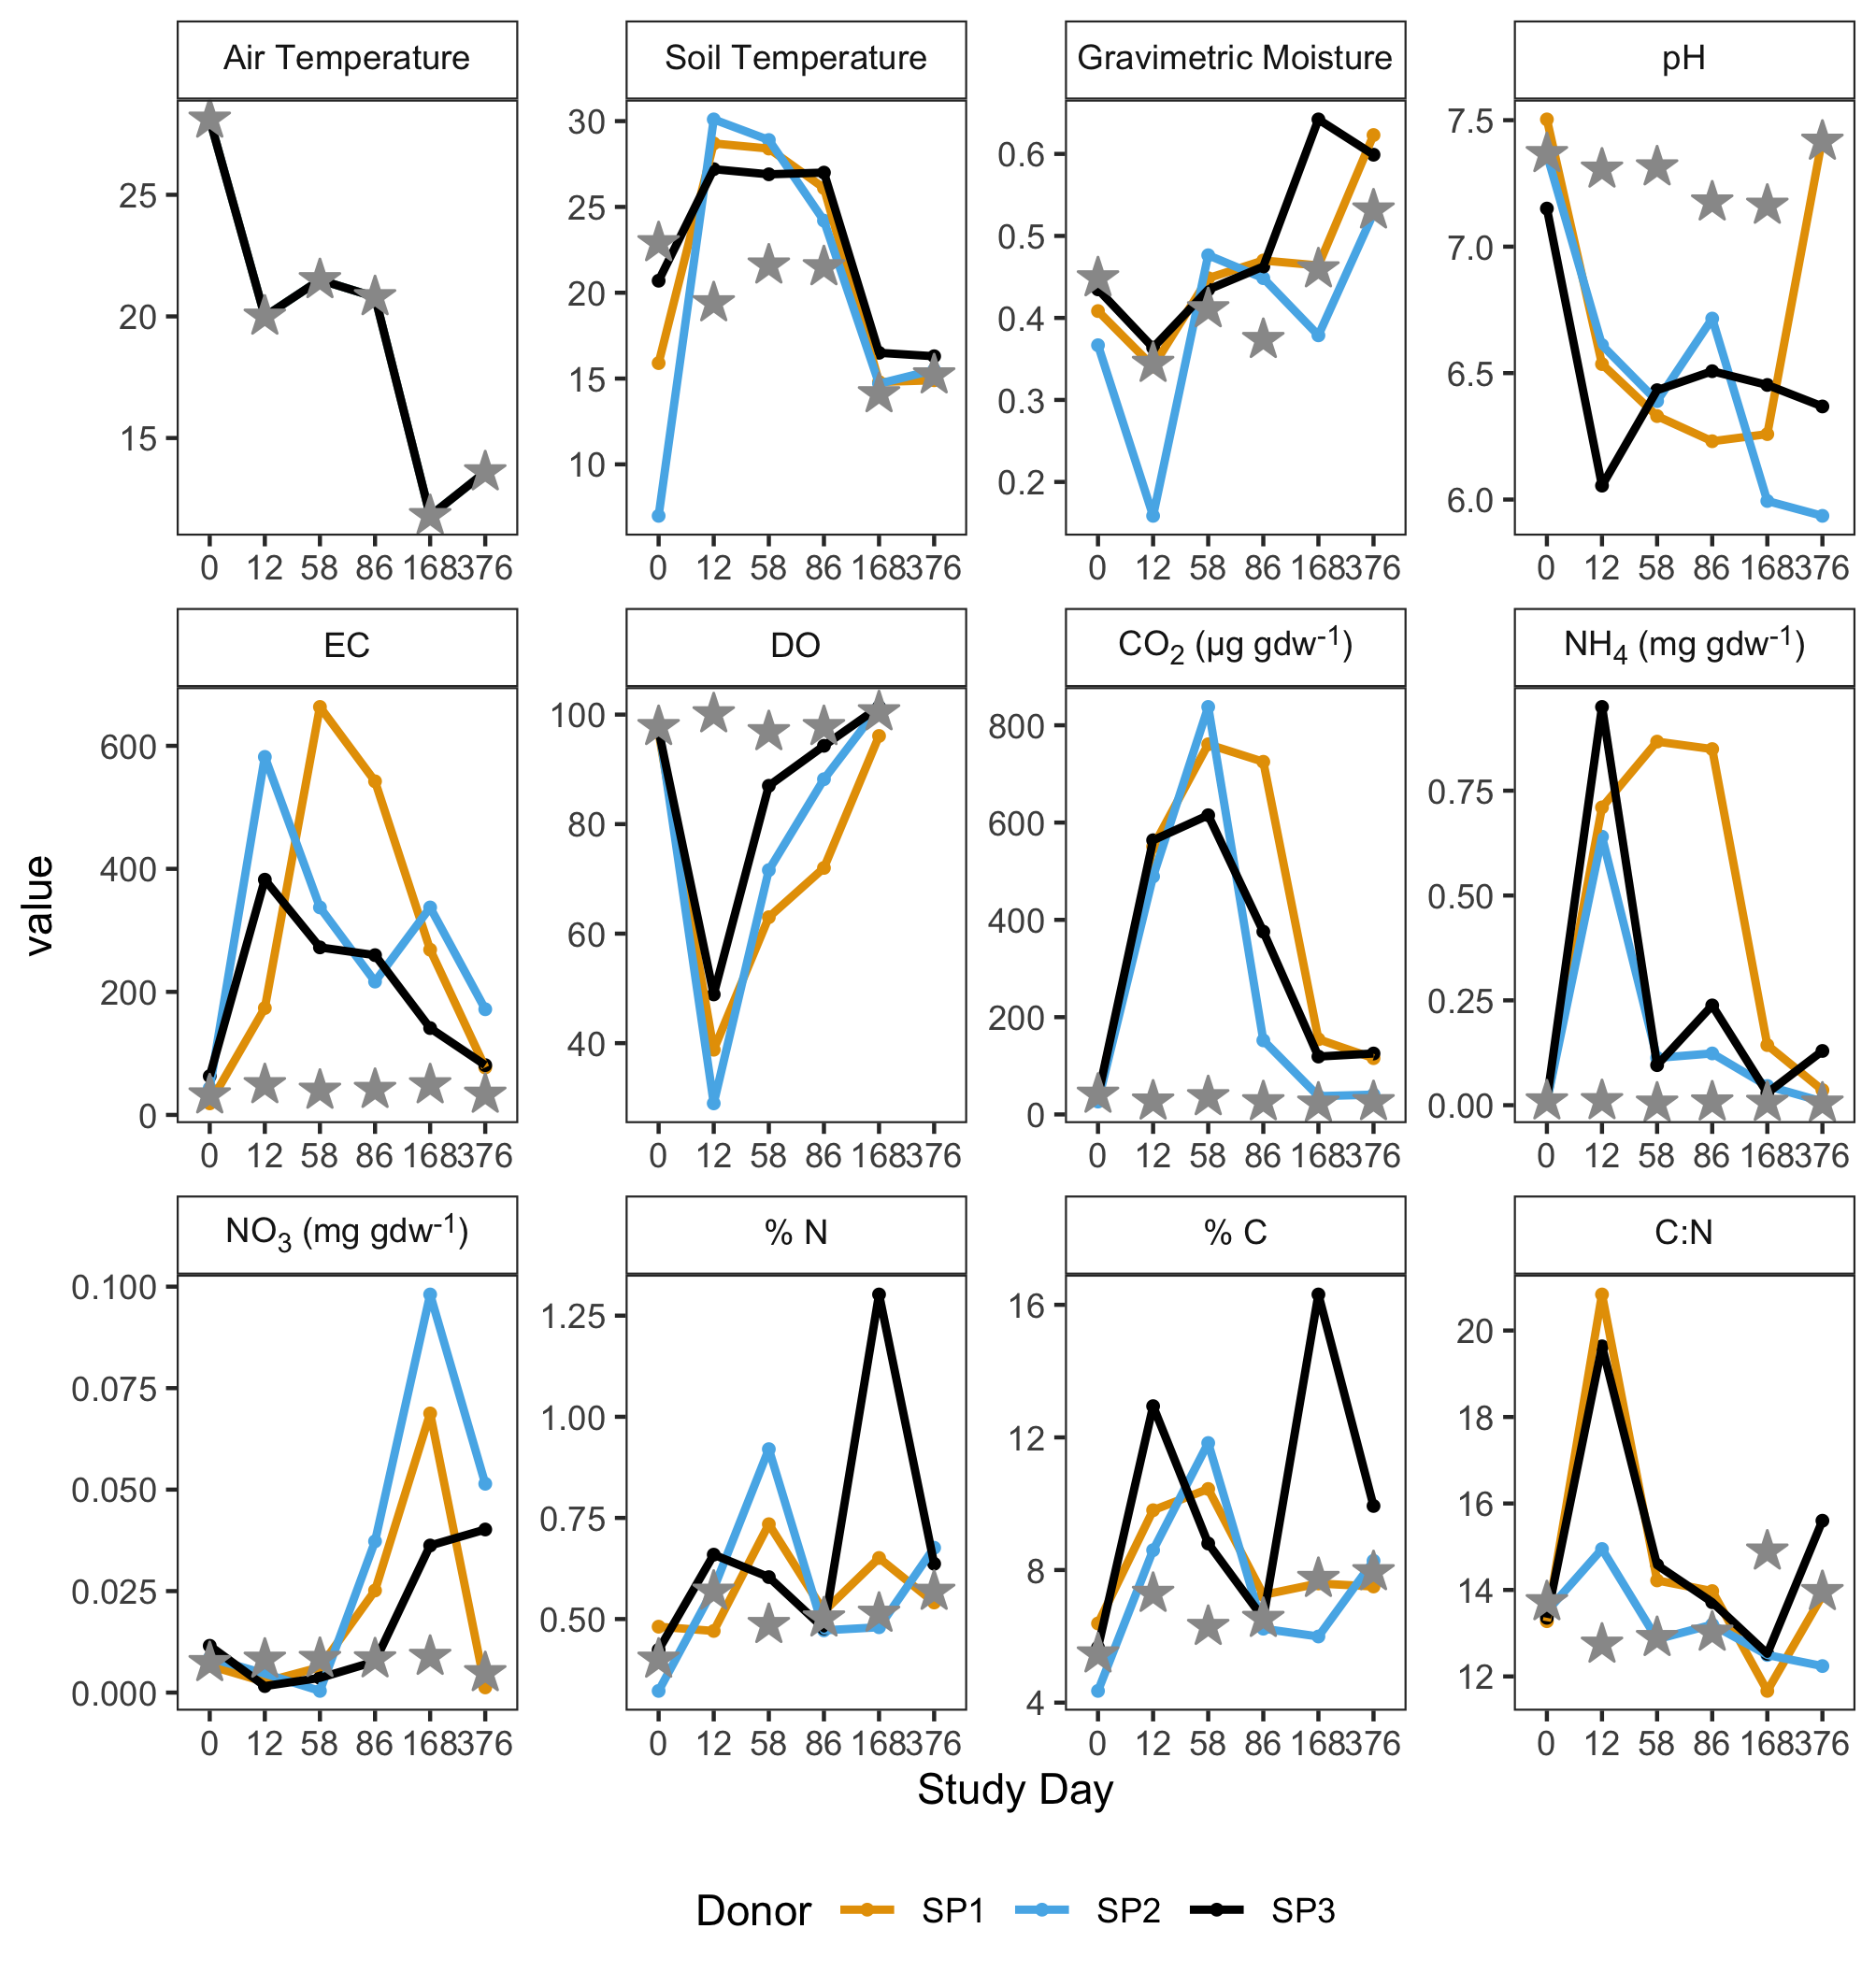
\includegraphics[keepaspectratio]{../../figures/soilchem_summary.png}}

Figure S1. Soil physiochemical parameters in decomposition soils during
the one-year study. Data is shown for each individual donor: SP1 (gold),
SP2 (blue), and SP2 (black). Values for the full 16 cm core samples were
estimated by summing values interface (0-1 cm) and core (0-16 cm)
reported by Taylor et al.~(2024) in 1:16 and 15:16 ratios, respectively.
Controls reported here are means of three experimental controls that
were unimpacted by decomposition and are represented by stars.

\pagebreak

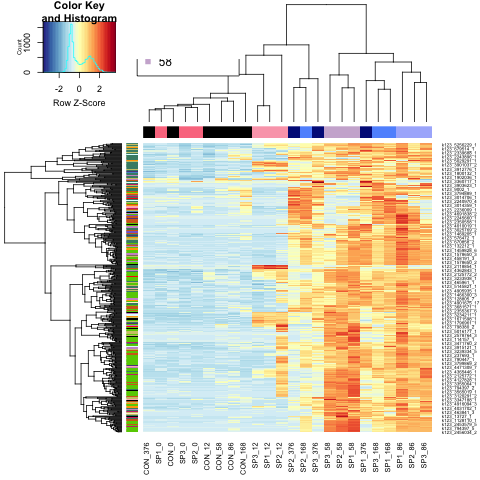
\includegraphics[width=1\textwidth]{../../figures/Fig_S2.png}

Figure S2. Hierarchical clustering heatmap showing the log counts per
million (CPM) of the top 500 most variable genes across samples.
Variable genes were determined by selecting genes with the highest
variance in gene expression. Samples are clustered along the x-axis
using Euclidean distances between samples and colored by study day.
Sample names denote donor (SP1, SP2, SP3) and sample day.

\pagebreak

Table S1. Permutational analysis of variance (PERMANOVA) results
identifying significant environmental parameters which explain some of
the variation in soil gene expression profiles. Environmental parameter
data is from Taylor et al.~(2024). Variables with p \textless{} 0.05 are
indicated in bold.

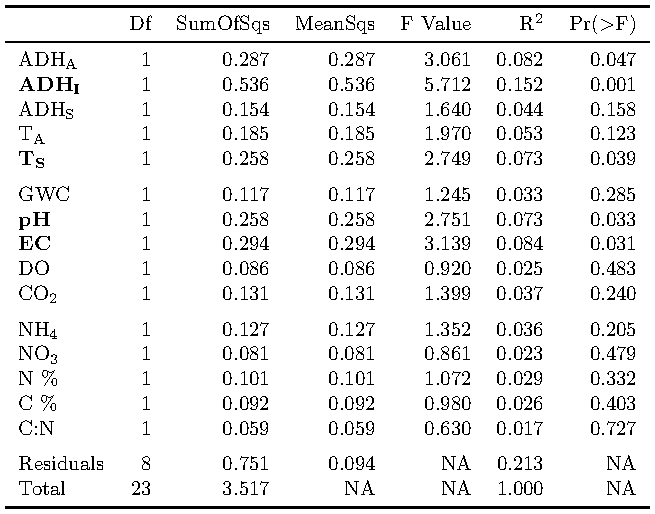
\includegraphics[scale=1.4,page=1]{../../tables/cca_permanova.pdf}

\pagebreak

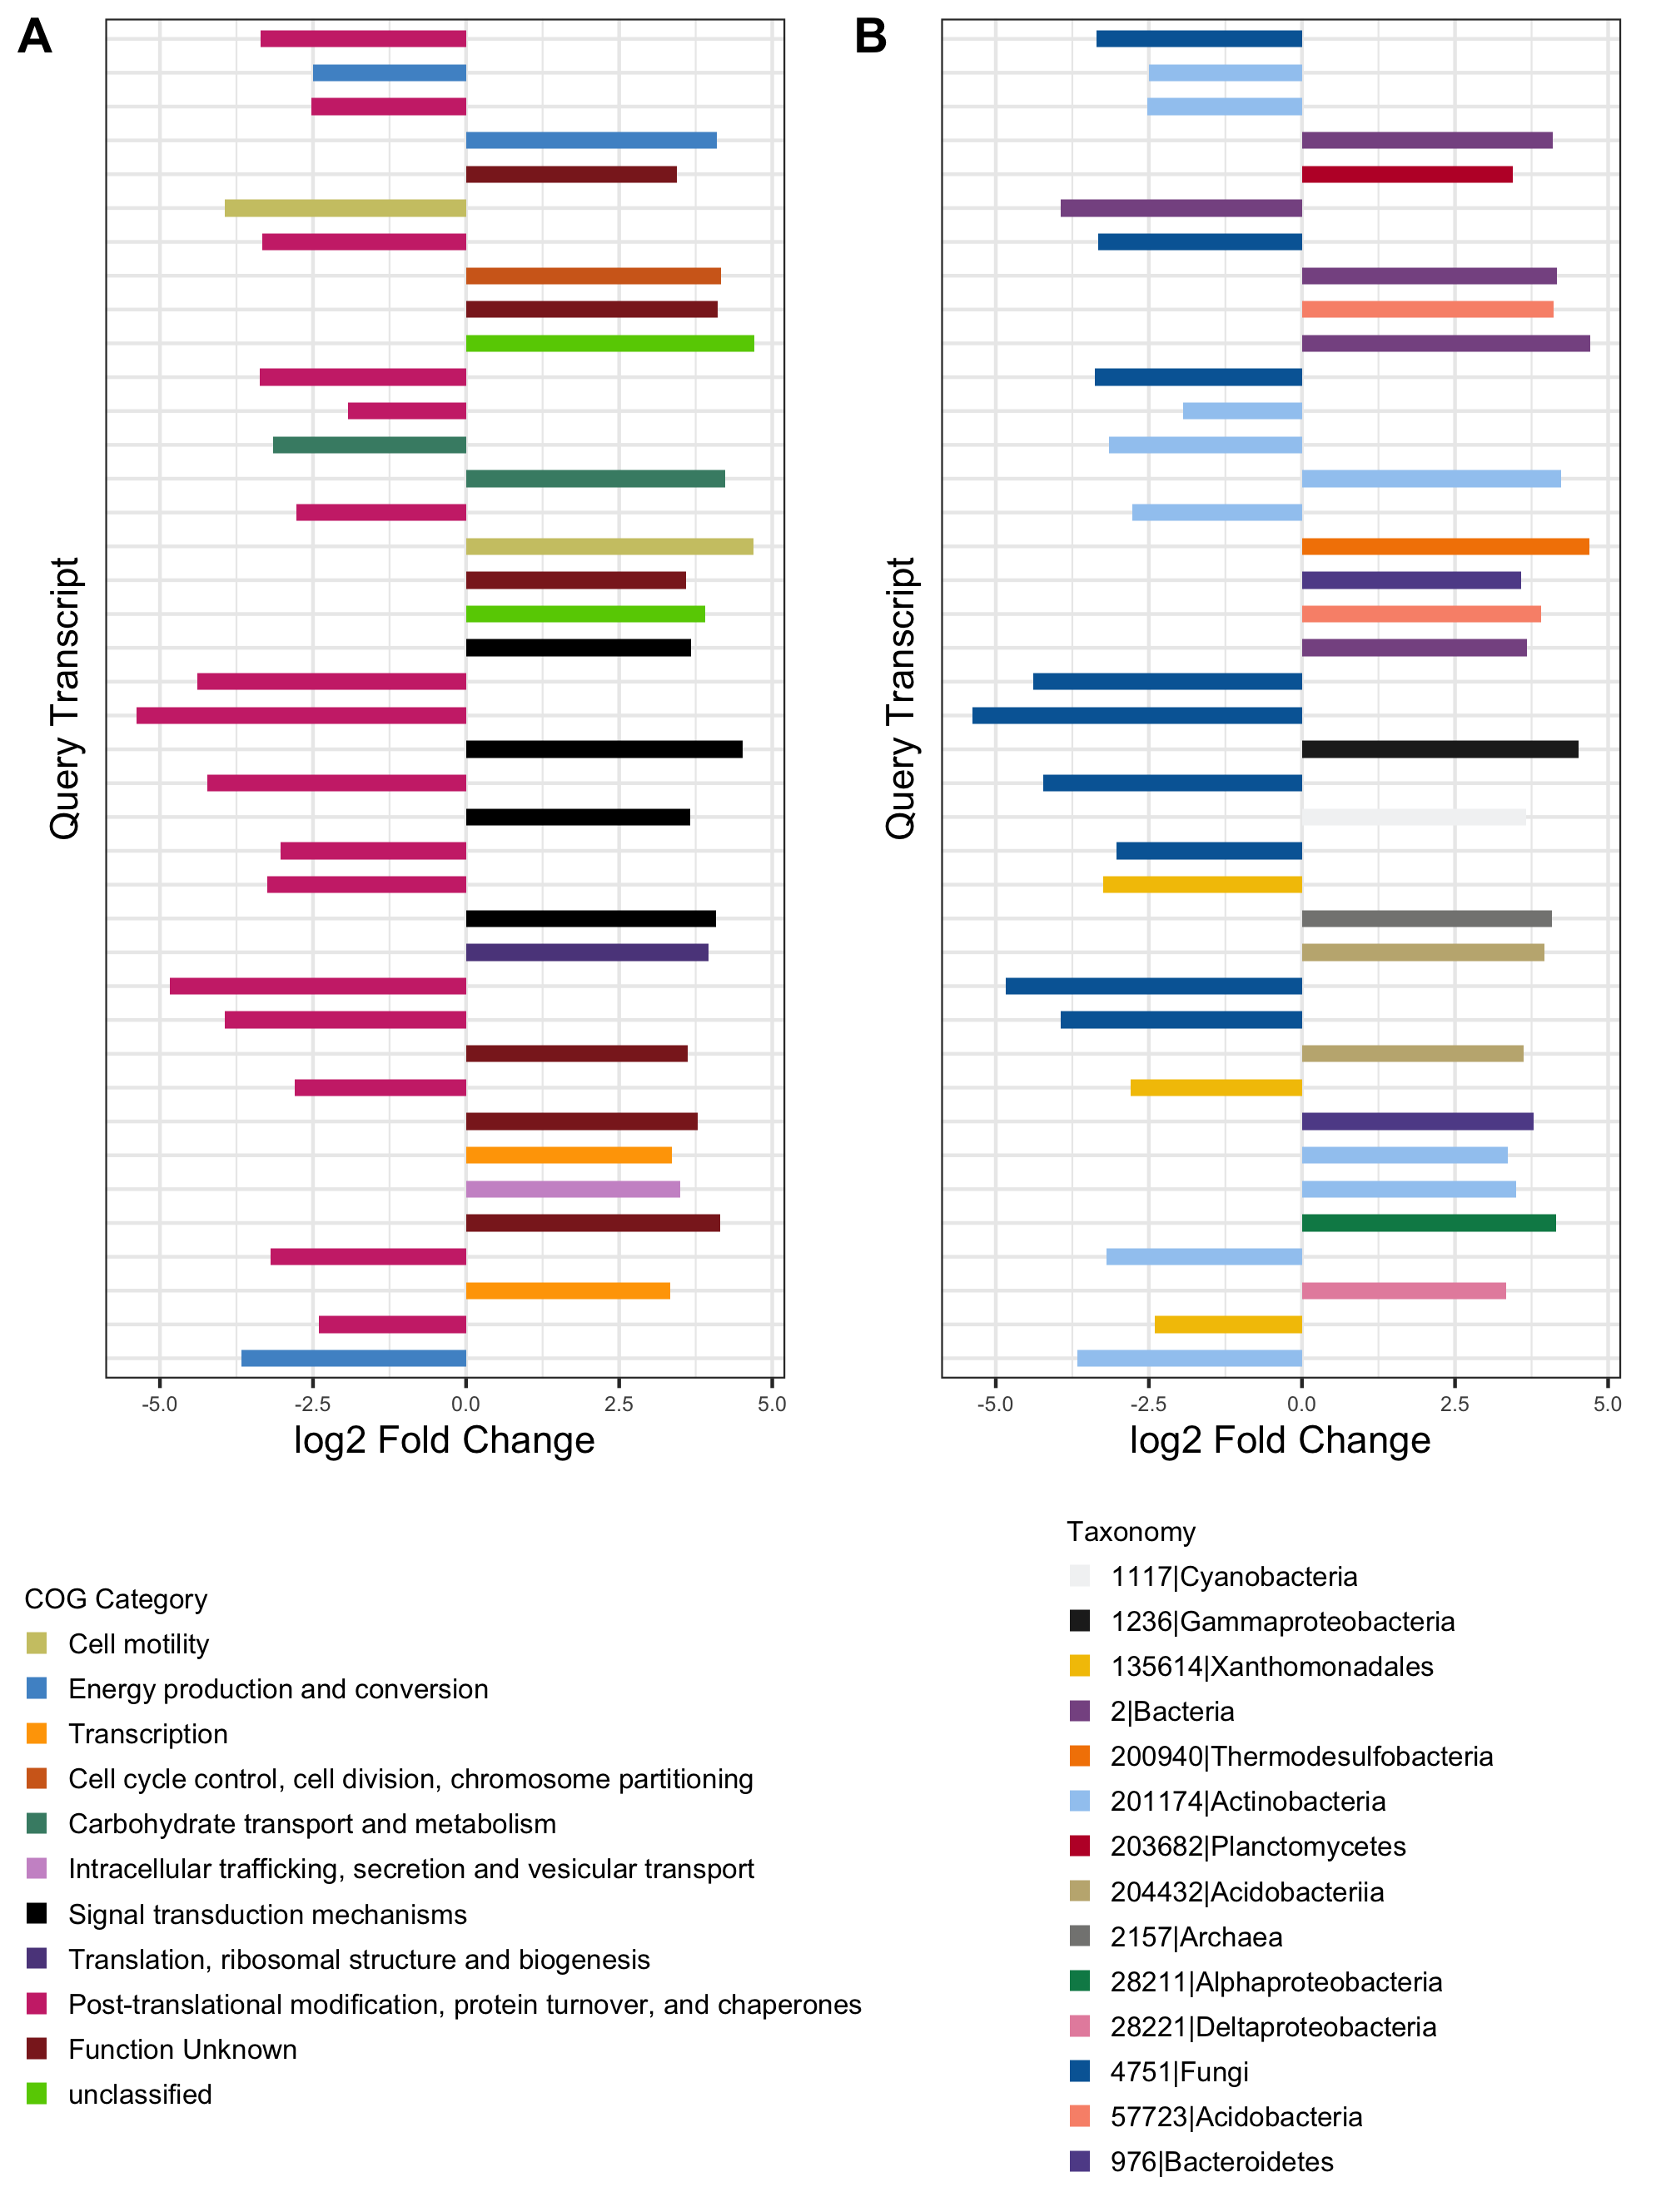
\includegraphics[width=0.88\textwidth]{../../figures/Trt_DE_top20_barplot.png}

Figure S3. Top 40 up- and down-regulated genes in controls relative to
decomposition soils across all study days, colored by COG functional
category (A) and taxonomic annotation (B). Positive values denote higher
expression in controls, while negative values are higher in
decomposition soils.

\pagebreak

\begin{landscape}

Table S2. Top 20 most significant up- and down-regulated gene queries,
determined by log2 fold change and adjusted p-values, in control
relative to decomposition soils. Positive log2 fold change values
represent genes whose expression was higher in control soils, while
negative log2 fold change values were higher in decomposition soils.
Taxonomic annotation, COG categories, gene description, gene names, and
EC were assigned via eggNOG-mapper.

\begin{longtable*}[t]{>{\raggedright\arraybackslash}p{6em}rrl>{\raggedright\arraybackslash}p{4em}>{\raggedright\arraybackslash}p{8em}>{\raggedright\arraybackslash}p{4em}>{\raggedright\arraybackslash}p{5em}}
\toprule
Query & Coefficient & p-Value & Taxonomic Annotation & COG Category & Description & Gene Name & EC\\
\midrule
\endfirsthead
\multicolumn{8}{@{}l}{\textit{(continued)}}\\
\toprule
Query & Coefficient & p-Value & Taxonomic Annotation & COG Category & Description & Gene Name & EC\\
\midrule
\endhead

\endfoot
\bottomrule
\endlastfoot
k123\_3586165\_1 & 4.699 & 0 & Thermodesulfobacteria & NU & Type II secretion system (T2SS), protein E, N-terminal domain & - & -\\
k123\_5240316\_1 & 3.444 & 0 & Planctomycetes & S & TIGRFAM type VI secretion protein, VC\_A0111 family & - & -\\
k123\_4233415\_1 & 4.708 & 0 & Bacteria & - & - & - & -\\
k123\_5247798\_1 & 4.101 & 0 & Bacteria & CO & amine dehydrogenase activity & - & -\\
k123\_1022852\_1 & 3.340 & 0 & Deltaproteobacteria & K & ROS/MUCR transcriptional regulator protein & - & -\\
\addlinespace
k123\_4454813\_1 & 4.159 & 0 & Bacteria & D & protein conserved in cyanobacteria & - & -\\
k123\_3793442\_4 & 4.229 & 0 & Actinobacteria & G & pfkB family carbohydrate kinase & kdgK & 2.7.1.45\\
k123\_3567914\_2 & 3.910 & 0 & Acidobacteria & - & - & - & -\\
k123\_3575243\_1 & 3.586 & 0 & Bacteroidetes & S & Protein of unknown function (DUF1501) & - & -\\
k123\_1456133\_1 & 3.496 & 0 & Actinobacteria & U & TadE-like protein & - & -\\
\addlinespace
k123\_1678879\_1 & 3.364 & 0 & Actinobacteria & K & DNA binding & - & -\\
k123\_1448646\_1 & 4.154 & 0 & Alphaproteobacteria & S & Type VI secretion system effector, Hcp & - & -\\
k123\_2582928\_1 & 3.665 & 0 & Cyanobacteria & T & Signal Transduction Histidine Kinase & - & -\\
k123\_4454279\_1 & 4.115 & 0 & Acidobacteria & S & Type VI secretion system effector, Hcp & - & -\\
k123\_2804786\_1 & 4.518 & 0 & Gammaproteobacteria & T & Domain present in phytochromes and cGMP-specific phosphodiesterases. & - & -\\
\addlinespace
k123\_1682627\_1 & 3.786 & 0 & Bacteroidetes & S & Protein of unknown function (DUF1800) & - & -\\
k123\_3238410\_1 & 3.678 & 0 & Bacteria & T & phosphoprotein phosphatase activity & - & 6.5.1.3\\
k123\_2360350\_2 & 3.954 & 0 & Acidobacteriia & J & One of the early assembly proteins it binds 23S rRNA. One of the proteins that surrounds the polypeptide exit tunnel on the outside of the ribosome. Forms the main docking site for trigger factor binding to the ribosome & rplW & -\\
k123\_244719\_2 & 4.077 & 0 & Archaea & T & Histidine kinase-, DNA gyrase B-, and HSP90-like ATPase & - & 2.7.7.65\\
k123\_1904408\_4 & 3.615 & 0 & Acidobacteriia & S & ASPIC and UnbV & - & -\\
\addlinespace
k123\_4681706\_1 & -3.333 & 0 & Fungi & O & Belongs to the heat shock protein 70 family & SSA2 & -\\
k123\_2129273\_1 & -3.939 & 0 & Fungi & O & Belongs to the heat shock protein 70 family & SSA2 & -\\
k123\_2784358\_1 & -4.226 & 0 & Fungi & O & Heat shock protein & HSP82 & -\\
k123\_2453574\_1 & -3.251 & 0 & Xanthomonadales & O & Part of a stress-induced multi-chaperone system, it is involved in the recovery of the cell from heat-induced damage, in cooperation with DnaK, DnaJ and GrpE & clpB & -\\
k123\_2580989\_1 & -3.034 & 0 & Fungi & O & MreB/Mbl protein & SSA2 & -\\
\addlinespace
k123\_784972\_1 & -3.361 & 0 & Fungi & O & Belongs to the heat shock protein 70 family & SSA2 & -\\
k123\_5131902\_2 & -3.945 & 0 & Bacteria & N & domain, Protein & - & 3.2.1.81,3.2.1.97\\
k123\_1897324\_1 & -2.804 & 0 & Xanthomonadales & O & Part of a stress-induced multi-chaperone system, it is involved in the recovery of the cell from heat-induced damage, in cooperation with DnaK, DnaJ and GrpE & clpB & -\\
k123\_1007534\_1 & -3.669 & 0 & Actinobacteria & C & Ferredoxin & fdxA & -\\
k123\_1119824\_1 & -3.191 & 0 & Actinobacteria & O & Heat shock 70 kDa protein & dnaK & -\\
\addlinespace
k123\_3696373\_1 & -2.768 & 0 & Actinobacteria & O & Prevents misfolding and promotes the refolding and proper assembly of unfolded polypeptides generated under stress conditions & groL2 & -\\
k123\_3023451\_1 & -5.388 & 0 & Fungi & O & Hsp90 protein & HSP82 & -\\
k123\_1018246\_1 & -2.400 & 0 & Xanthomonadales & O & Part of a stress-induced multi-chaperone system, it is involved in the recovery of the cell from heat-induced damage, in cooperation with DnaK, DnaJ and GrpE & clpB & -\\
k123\_4142344\_1 & -3.376 & 0 & Fungi & O & Hsp90 protein & HSP82 & -\\
k123\_3914888\_1 & -3.146 & 0 & Actinobacteria & G & Phosphoketolase & - & 4.1.2.22,4.1.2.9\\
\addlinespace
k123\_3122150\_1 & -4.387 & 0 & Fungi & O & Heat shock protein & HSP82 & -\\
k123\_4027381\_1 & -1.934 & 0 & Actinobacteria & O & Part of a stress-induced multi-chaperone system, it is involved in the recovery of the cell from heat-induced damage, in cooperation with DnaK, DnaJ and GrpE & clpB & -\\
k123\_572232\_1 & -2.504 & 0 & Actinobacteria & C & 4Fe-4S dicluster domain & fadF & -\\
k123\_559972\_1 & -2.527 & 0 & Actinobacteria & O & Heat shock 70 kDa protein & dnaK & -\\
k123\_2243380\_1 & -4.837 & 0 & Fungi & O & Belongs to the heat shock protein 70 family & SSA2 & -\\*
\end{longtable*}

\pagebreak

Table S3. Top 10 most significant up- and down-regulated transcripts,
determined by log2 fold change and adjusted p-values, for each
sequential timepoint comparison. Positive log2 fold change values
represent genes whose expression was higher in the later decomposition
timepoint soils, while negative log2 fold change values are higher in
earlier decomposition timepoint soils. Taxonomic annotation, COG
categories, gene names, and EC were assigned via eggNOG-mapper. The
comparison column distinguishes each timepoint comparison.

\begingroup\fontsize{10}{12}\selectfont

\begin{longtable*}[t]{l>{\raggedright\arraybackslash}p{4.5em}>{\raggedleft\arraybackslash}p{4.5em}l>{\raggedright\arraybackslash}p{10em}>{\raggedright\arraybackslash}p{4em}>{\raggedright\arraybackslash}p{8em}>{\raggedright\arraybackslash}p{4em}>{\raggedright\arraybackslash}p{4em}}
\toprule
Query & Comparison & Coefficient & p-Value & Taxonomic Annotation & COG Category & Description & Gene Name & EC\\
\midrule
\endfirsthead
\multicolumn{9}{@{}l}{\textit{(continued)}}\\
\toprule
Query & Comparison & Coefficient & p-Value & Taxonomic Annotation & COG Category & Description & Gene Name & EC\\
\midrule
\endhead

\endfoot
\bottomrule
\endlastfoot
k123\_3351426\_1 & 0-12 & 11.410 & < 0.001 & Clostridia & S & Flavin reductase like domain & - & -\\
k123\_3689959\_6 & 0-12 & 12.863 & < 0.001 & Bacilli & GM & NmrA-like family & - & -\\
k123\_1682409\_1 & 0-12 & 12.514 & < 0.001 & Bacilli & C & Oxidoreductase required for the transfer of electrons from pyruvate to flavodoxin & nifJ & 1.2.7.1\\
k123\_4131385\_2 & 0-12 & 11.768 & < 0.001 & Bacilli & M & Domain of unknown function (DUF5011) & - & -\\
k123\_3474748\_6 & 0-12 & 11.248 & < 0.001 & Bacilli & E & ABC transporter substrate-binding protein & oppA & -\\
\addlinespace
k123\_2018420\_1 & 0-12 & 11.126 & < 0.001 & Bacilli & G & PTS fructose transporter subunit IIC & fruA & 2.7.1.202\\
k123\_4134106\_1 & 0-12 & 10.776 & < 0.001 & Bacilli & C & e3 binding domain & pdhC & 2.3.1.12\\
k123\_2451258\_1 & 0-12 & 12.572 & < 0.001 & Clostridia & M & S-layer homology domain & - & -\\
k123\_3683359\_3 & 0-12 & 12.858 & < 0.001 & Bacilli & P & P-type ATPase & copA & 3.6.3.54\\
k123\_2018420\_3 & 0-12 & 9.998 & < 0.001 & Bacilli & GKT & Transcriptional antiterminator & manR & -\\
\addlinespace
k123\_4030449\_2 & 0-12 & -7.201 & < 0.001 & Gammaproteobacteria & C & PFAM blue (type 1) copper domain protein & - & -\\
k123\_1903136\_2 & 0-12 & -6.769 & < 0.001 & Actinobacteria & Q & Taurine catabolism dioxygenase TauD, TfdA family & - & 1.14.11.17\\
k123\_4017556\_1 & 0-12 & -6.740 & < 0.001 & Betaproteobacteria & Q & Taurine dioxygenase & - & 1.14.11.17\\
k123\_2470867\_1 & 0-12 & -6.354 & < 0.001 & Actinobacteria & Q & taurine catabolism dioxygenase & tauD & 1.14.11.17\\
k123\_2231885\_1 & 0-12 & -5.426 & < 0.001 & Actinobacteria & E & ABC-type branched-chain amino acid transport & - & -\\
\addlinespace
k123\_1903136\_1 & 0-12 & -5.513 & < 0.001 & Actinobacteria & K & Bacterial regulatory proteins, tetR family & - & -\\
k123\_3697194\_1 & 0-12 & -5.446 & < 0.001 & Actinobacteria & Q & Taurine catabolism dioxygenase TauD, TfdA family & tauD & 1.14.11.17\\
k123\_4238273\_1 & 0-12 & -6.106 & < 0.001 & Deltaproteobacteria & S & Part of the outer membrane protein assembly complex, which is involved in assembly and insertion of beta-barrel proteins into the outer membrane & - & -\\
k123\_2680211\_1 & 0-12 & -5.155 & < 0.001 & Proteobacteria & Q & Multicopper oxidase & - & 1.16.3.3\\
k123\_4688925\_2 & 0-12 & -6.014 & < 0.001 & Betaproteobacteria & C & D-arabinono-1,4-lactone oxidase & - & -\\
\addlinespace
k123\_785677\_1 & 12-58 & 12.106 & < 0.001 & Betaproteobacteria & J & One of the primary rRNA binding proteins, it binds directly near the 3'-end of the 23S rRNA, where it nucleates assembly of the 50S subunit & rplC & -\\
k123\_2456034\_2 & 12-58 & 11.226 & < 0.001 & Betaproteobacteria & J & Forms part of the polypeptide exit tunnel & rplD & -\\
k123\_3024550\_1 & 12-58 & 10.815 & < 0.001 & Betaproteobacteria & J & This is one of the proteins that binds to the 5S RNA in the ribosome where it forms part of the central protuberance & ctc & -\\
k123\_1916443\_2 & 12-58 & 11.317 & < 0.001 & Betaproteobacteria & J & Binds directly to 23S ribosomal RNA and is necessary for the in vitro assembly process of the 50S ribosomal subunit. It is not involved in the protein synthesizing functions of that subunit & rplT & -\\
k123\_794397\_5 & 12-58 & 12.046 & < 0.001 & Betaproteobacteria & J & Ribosomal protein L17 & rplQ & -\\
\addlinespace
k123\_1010408\_1 & 12-58 & 11.827 & < 0.001 & Betaproteobacteria & J & This is 1 of the proteins that binds and probably mediates the attachment of the 5S RNA into the large ribosomal subunit, where it forms part of the central protuberance. In the 70S ribosome it contacts protein S13 of the 30S subunit (bridge B1b), connecting the 2 subunits & rplE & -\\
k123\_1115623\_7 & 12-58 & 10.795 & < 0.001 & Betaproteobacteria & JKL & Belongs to the DEAD box helicase family & rhlE1 & -\\
k123\_3802697\_1 & 12-58 & 10.705 & < 0.001 & Betaproteobacteria & JKL & Belongs to the DEAD box helicase family & rhlE1 & -\\
k123\_5130820\_1 & 12-58 & 11.586 & < 0.001 & Betaproteobacteria & JKL & Belongs to the DEAD box helicase family & rhlE1 & -\\
k123\_2572977\_1 & 12-58 & 11.374 & < 0.001 & Betaproteobacteria & U & The central subunit of the protein translocation channel SecYEG. Consists of two halves formed by TMs 1-5 and 6-10. These two domains form a lateral gate at the front which open onto the bilayer between TMs 2 and 7, and are clamped together by SecE at the back. The channel is closed by both a pore ring composed of hydrophobic SecY resides and a short helix (helix 2A) on the extracellular side of the membrane which forms a plug. The plug probably moves laterally to allow the channel to open. The ring and the pore may move independently & secY & -\\
\addlinespace
k123\_3351426\_1 & 12-58 & -10.845 & < 0.001 & Clostridia & S & Flavin reductase like domain & - & -\\
k123\_3689959\_6 & 12-58 & -12.298 & < 0.001 & Bacilli & GM & NmrA-like family & - & -\\
k123\_4131385\_2 & 12-58 & -11.203 & < 0.001 & Bacilli & M & Domain of unknown function (DUF5011) & - & -\\
k123\_1682409\_1 & 12-58 & -11.434 & < 0.001 & Bacilli & C & Oxidoreductase required for the transfer of electrons from pyruvate to flavodoxin & nifJ & 1.2.7.1\\
k123\_3028891\_1 & 12-58 & -10.738 & < 0.001 & Clostridia & K & PFAM flavin reductase & - & -\\
\addlinespace
k123\_2018420\_3 & 12-58 & -9.433 & < 0.001 & Bacilli & GKT & Transcriptional antiterminator & manR & -\\
k123\_3469192\_2 & 12-58 & -9.634 & < 0.001 & Clostridia & T & S-layer homology domain & - & -\\
k123\_3683359\_3 & 12-58 & -11.778 & < 0.001 & Bacilli & P & P-type ATPase & copA & 3.6.3.54\\
k123\_335030\_2 & 12-58 & -11.417 & < 0.001 & Bacilli & C & Iron-containing alcohol dehydrogenase & adhB & 1.1.1.1,1.1.1.202\\
k123\_3012292\_1 & 12-58 & -9.296 & < 0.001 & Bacilli & S & Putative neutral zinc metallopeptidase & yugP & -\\
\addlinespace
k123\_3581297\_1 & 58-86 & 8.049 & < 0.001 & Fungi & - & - & - & -\\
k123\_133381\_1 & 58-86 & 8.362 & < 0.001 & Betaproteobacteria & C & anaerobic respiration & - & 1.7.2.6\\
k123\_3681927\_1 & 58-86 & 8.474 & < 0.001 & Betaproteobacteria & C & Cytochrome C oxidase subunit II, periplasmic domain & - & 1.9.3.1\\
k123\_4461993\_6 & 58-86 & 10.379 & < 0.001 & Bacteroidetes & S & Tetratricopeptide repeat protein & - & -\\
k123\_1691746\_1 & 58-86 & 8.748 & < 0.001 & Rhodospirillales & C & NDH-1 shuttles electrons from NADH, via FMN and iron- sulfur (Fe-S) centers, to quinones in the respiratory chain. The immediate electron acceptor for the enzyme in this species is believed to be ubiquinone. Couples the redox reaction to proton translocation (for every two electrons transferred, four hydrogen ions are translocated across the cytoplasmic membrane), and thus conserves the redox energy in a proton gradient. This subunit may bind ubiquinone & nuoH & 1.6.5.3\\
\addlinespace
k123\_1674520\_1 & 58-86 & 8.655 & < 0.001 & Alphaproteobacteria & C & Produces ATP from ADP in the presence of a proton gradient across the membrane. The alpha chain is a regulatory subunit & atpA & 3.6.3.14\\
k123\_4907595\_1 & 58-86 & 8.469 & < 0.001 & Oceanospirillales & J & Belongs to the universal ribosomal protein uS2 family & rpsB & -\\
k123\_788629\_1 & 58-86 & 8.018 & < 0.001 & Bacteroidetes & PT & COGs COG3712 Fe2 -dicitrate sensor membrane component & - & -\\
k123\_784141\_1 & 58-86 & 6.602 & < 0.001 & Bacteroidetes & - & - & - & -\\
k123\_2678388\_2 & 58-86 & 7.966 & < 0.001 & Betaproteobacteria & C & Subunits I and II form the functional core of the enzyme complex. Electrons originating in cytochrome c are transferred via heme a and Cu(A) to the binuclear center formed by heme a3 and Cu(B) & coxB & 1.9.3.1\\
\addlinespace
k123\_903075\_1 & 58-86 & -7.906 & < 0.001 & Bacteroidetes & - & - & - & -\\
k123\_2460567\_2 & 58-86 & -7.060 & < 0.001 & Bacteroidetes & S & Functions as a peptidoglycan terminase that cleaves nascent peptidoglycan strands endolytically to terminate their elongation & mltG & -\\
k123\_680086\_2 & 58-86 & -6.939 & < 0.001 & Bacteria & - & - & - & -\\
k123\_3353720\_2 & 58-86 & -7.036 & < 0.001 & Bacteroidetes & U & Preprotein translocase SecG subunit & secG & -\\
k123\_4342821\_1 & 58-86 & -6.571 & < 0.001 & Bacteroidetes & CO & Redoxin & - & -\\
\addlinespace
k123\_680086\_6 & 58-86 & -6.695 & < 0.001 & Bacteroidetes & G & Sad1 / UNC-like C-terminal & - & -\\
k123\_3687116\_4 & 58-86 & -6.677 & < 0.001 & Bacteroidetes & S & Belongs to the pirin family & yhhW & -\\
k123\_349053\_1 & 58-86 & -6.992 & < 0.001 & Bacteroidetes & F & Catalyzes the conversion of inosine 5'-phosphate (IMP) to xanthosine 5'-phosphate (XMP), the first committed and rate- limiting step in the de novo synthesis of guanine nucleotides, and therefore plays an important role in the regulation of cell growth & guaB & 1.1.1.205\\
k123\_2348950\_2 & 58-86 & -6.358 & < 0.001 & Bacteroidetes & O & Heat shock protein & - & -\\
k123\_1004837\_2 & 58-86 & -7.162 & < 0.001 & Bacteroidetes & S & Fimbrillin-like & - & -\\
\addlinespace
k123\_465331\_1 & 86-168 & 6.832 & < 0.001 & Bacteroidetes & M & Pkd domain containing protein & - & -\\
k123\_1247591\_2 & 86-168 & 6.662 & < 0.001 & Xanthomonadales & - & - & - & -\\
k123\_356907\_3 & 86-168 & 7.008 & < 0.001 & Actinobacteria & I & Fatty acid desaturase & desA3\_2 & -\\
k123\_1802620\_3 & 86-168 & 6.775 & < 0.001 & Actinobacteria & S & Protein of unknown function (DUF1360) & - & -\\
k123\_4137171\_1 & 86-168 & 7.254 & < 0.001 & Actinobacteria & U & WD40-like Beta Propeller Repeat & - & -\\
\addlinespace
k123\_1449660\_1 & 86-168 & 7.112 & < 0.001 & Actinobacteria & S & LVIVD repeat & - & -\\
k123\_3015796\_1 & 86-168 & 6.131 & < 0.001 & Actinobacteria & S & Tetratricopeptide repeat & - & -\\
k123\_4469568\_1 & 86-168 & 8.516 & < 0.001 & Gammaproteobacteria & NU & Pilin (bacterial filament) & pilA & -\\
k123\_4013561\_1 & 86-168 & 6.723 & < 0.001 & Xanthomonadales & N & Required for morphogenesis and for the elongation of the flagellar filament by facilitating polymerization of the flagellin monomers at the tip of growing filament. Forms a capping structure, which prevents flagellin subunits (transported through the central channel of the flagellum) from leaking out without polymerization at the distal end & fliD & -\\
k123\_4136401\_2 & 86-168 & 6.097 & < 0.001 & Actinobacteria & O & FKBP-type peptidyl-prolyl cis-trans isomerase & fkbB & 5.2.1.8\\
\addlinespace
k123\_2576445\_1 & 86-168 & -7.806 & < 0.001 & Xanthomonadales & M & Belongs to the ompA family & mopB & -\\
k123\_2013370\_2 & 86-168 & -7.409 & < 0.001 & Gammaproteobacteria & S & Protein of unknown function (DUF1471) & - & -\\
k123\_1784040\_1 & 86-168 & -7.539 & < 0.001 & Clostridia & L & PFAM Reverse transcriptase (RNA-dependent DNA polymerase) & - & -\\
k123\_2784492\_8 & 86-168 & -7.104 & < 0.001 & Actinobacteria & Q & Amidohydrolase family & - & -\\
k123\_1671881\_1 & 86-168 & -7.712 & < 0.001 & Bacteroidetes & P & von Willebrand factor, type A & - & -\\
\addlinespace
k123\_115662\_2 & 86-168 & -8.927 & < 0.001 & Bacilli & C & succinate dehydrogenase & sdhA & 1.3.5.1,1.3.5.4\\
k123\_2013542\_1 & 86-168 & -7.286 & < 0.001 & Betaproteobacteria & S & Domain of unknown function (DUF4148) & - & -\\
k123\_784141\_1 & 86-168 & -6.401 & < 0.001 & Bacteroidetes & - & - & - & -\\
k123\_126934\_1 & 86-168 & -8.876 & < 0.001 & Bacteroidetes & M & Belongs to the membrane fusion protein (MFP) (TC 8.A.1) family & - & -\\
k123\_3912958\_2 & 86-168 & -7.098 & < 0.001 & Bacteroidetes & C & cytochrome c oxidase & ccoG & -\\
\addlinespace
k123\_4347668\_1 & 168-376 & 7.985 & < 0.001 & Archaea & - & - & - & -\\
k123\_2010423\_2 & 168-376 & 8.457 & < 0.001 & Acidobacteria & J & Forms part of the ribosomal stalk, playing a central role in the interaction of the ribosome with GTP-bound translation factors & rplJ & -\\
k123\_4021403\_1 & 168-376 & 6.597 & < 0.001 & Acidobacteria & O & Prevents misfolding and promotes the refolding and proper assembly of unfolded polypeptides generated under stress conditions & groL & -\\
k123\_2899693\_1 & 168-376 & 6.546 & < 0.001 & Acidobacteria & O & Belongs to the ClpA ClpB family & - & -\\
k123\_461276\_1 & 168-376 & 9.975 & < 0.001 & Bacteria & N & domain, Protein & - & -\\
\addlinespace
k123\_13363\_1 & 168-376 & 6.773 & < 0.001 & Acidobacteria & O & Prevents misfolding and promotes the refolding and proper assembly of unfolded polypeptides generated under stress conditions & groL & -\\
k123\_3585893\_1 & 168-376 & 6.944 & < 0.001 & Acidobacteria & K & DNA-dependent RNA polymerase catalyzes the transcription of DNA into RNA using the four ribonucleoside triphosphates as substrates & rpoC & 2.7.7.6\\
k123\_3020221\_1 & 168-376 & 7.640 & < 0.001 & Xanthomonadales & - & - & - & -\\
k123\_4015238\_2 & 168-376 & 8.717 & < 0.001 & Acidobacteria & U & MotA TolQ ExbB proton channel & - & -\\
k123\_4017681\_1 & 168-376 & 8.220 & < 0.001 & Acidobacteria & J & Binds the lower part of the 30S subunit head. Binds mRNA in the 70S ribosome, positioning it for translation & rpsC & -\\
\addlinespace
k123\_465331\_1 & 168-376 & -7.066 & < 0.001 & Bacteroidetes & M & Pkd domain containing protein & - & -\\
k123\_4458935\_1 & 168-376 & -7.201 & < 0.001 & Epsilonproteobacteria & Q & calcium- and calmodulin-responsive adenylate cyclase activity & - & -\\
k123\_5025476\_3 & 168-376 & -8.470 & < 0.001 & Actinobacteria & G & phosphocarrier protein hpr & ptsH & -\\
k123\_1114482\_1 & 168-376 & -6.397 & < 0.001 & Bacteroidetes & MU & Outer membrane efflux protein & - & -\\
k123\_4360823\_3 & 168-376 & -6.013 & < 0.001 & Gammaproteobacteria & IQ & KR domain & - & 1.1.1.159\\
\addlinespace
k123\_3135574\_1 & 168-376 & -7.251 & < 0.001 & Actinobacteria & K & transcriptional regulator (DeoR family) & fruR & -\\
k123\_3354064\_4 & 168-376 & -6.628 & < 0.001 & Actinobacteria & G & Bacterial extracellular solute-binding protein & - & -\\
k123\_2683111\_1 & 168-376 & -6.487 & < 0.001 & Actinobacteria & G & L-arabinose isomerase & - & 5.3.1.4\\
k123\_4463835\_2 & 168-376 & -6.188 & < 0.001 & Actinobacteria & K & DNA-templated transcription, initiation & - & -\\
k123\_2915236\_1 & 168-376 & -7.060 & < 0.001 & Actinobacteria & M & probably involved in cell wall & - & -\\*
\end{longtable*}
\endgroup{}

\end{landscape}

\pagebreak

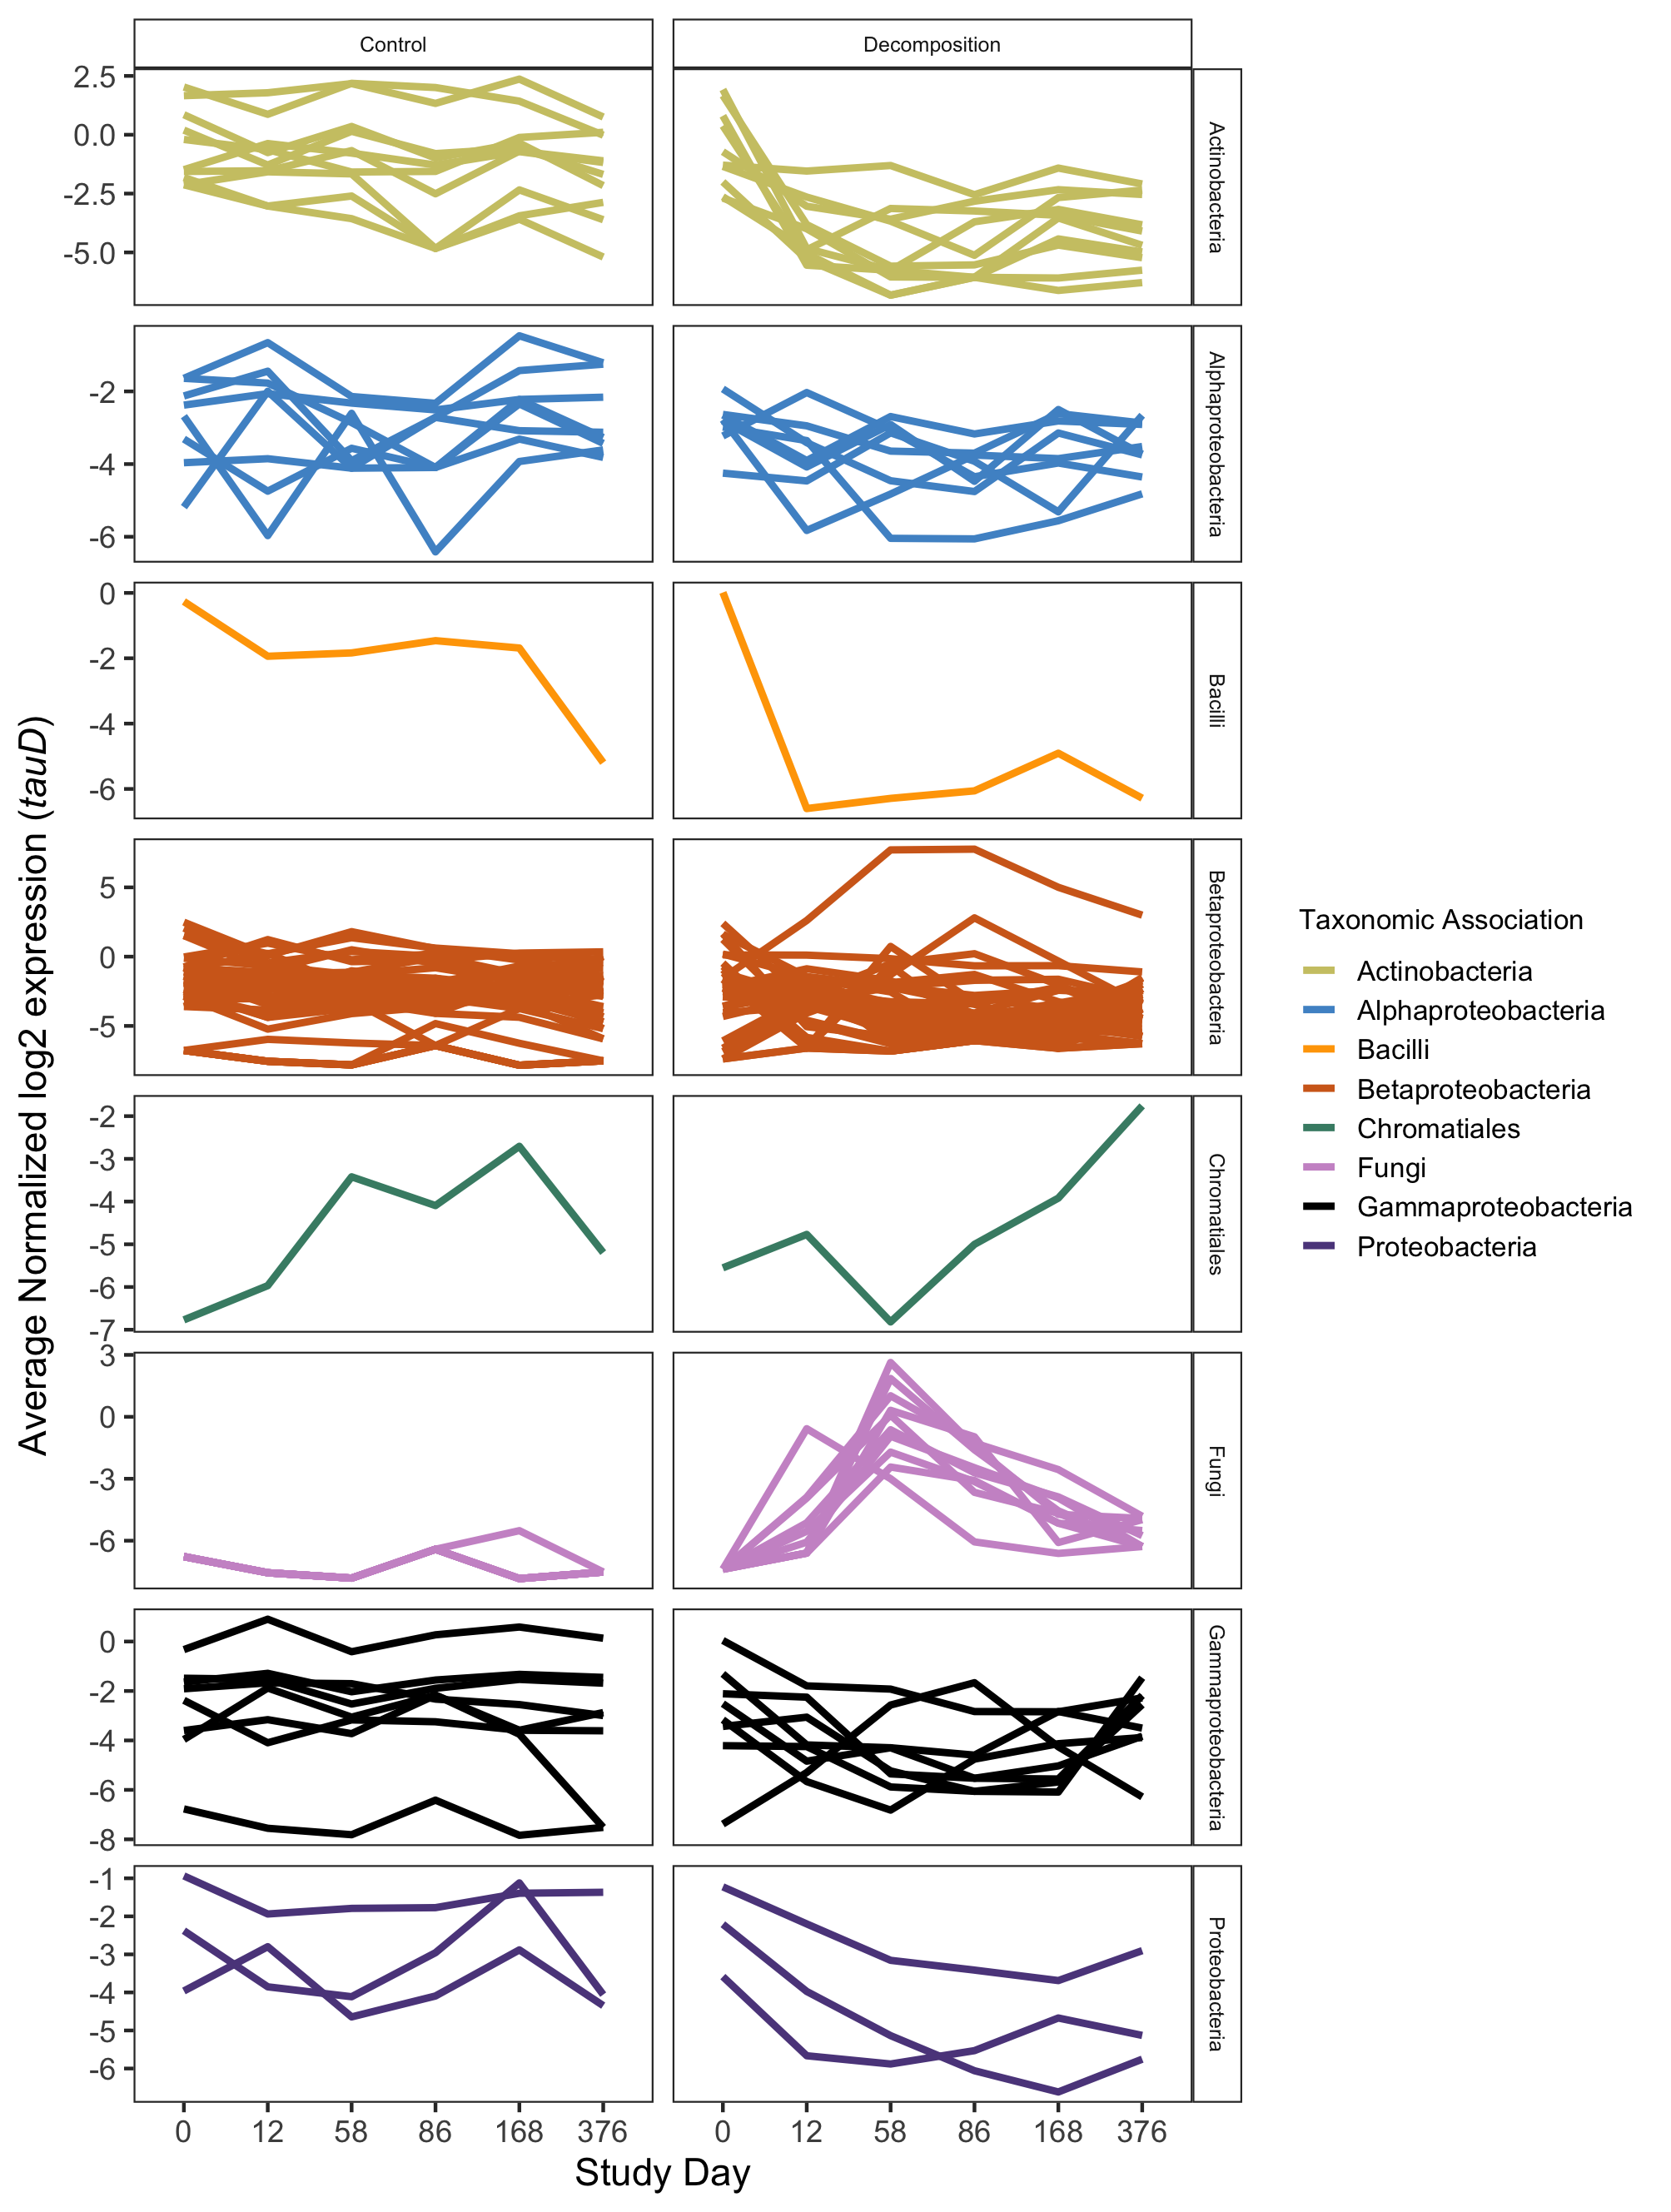
\includegraphics[width=0.9\textwidth]{../../figures/tauD_nlog2_taxonomy.png}

Figure S4. Mean normalized log2 expression of \emph{tauD} genes by
taxonomic association (color) in control and decomposition soils at each
study day. Each line represents one \emph{tauD} gene query, while color
denotes taxonomic association as determined by eggNOG-mapper.

\pagebreak

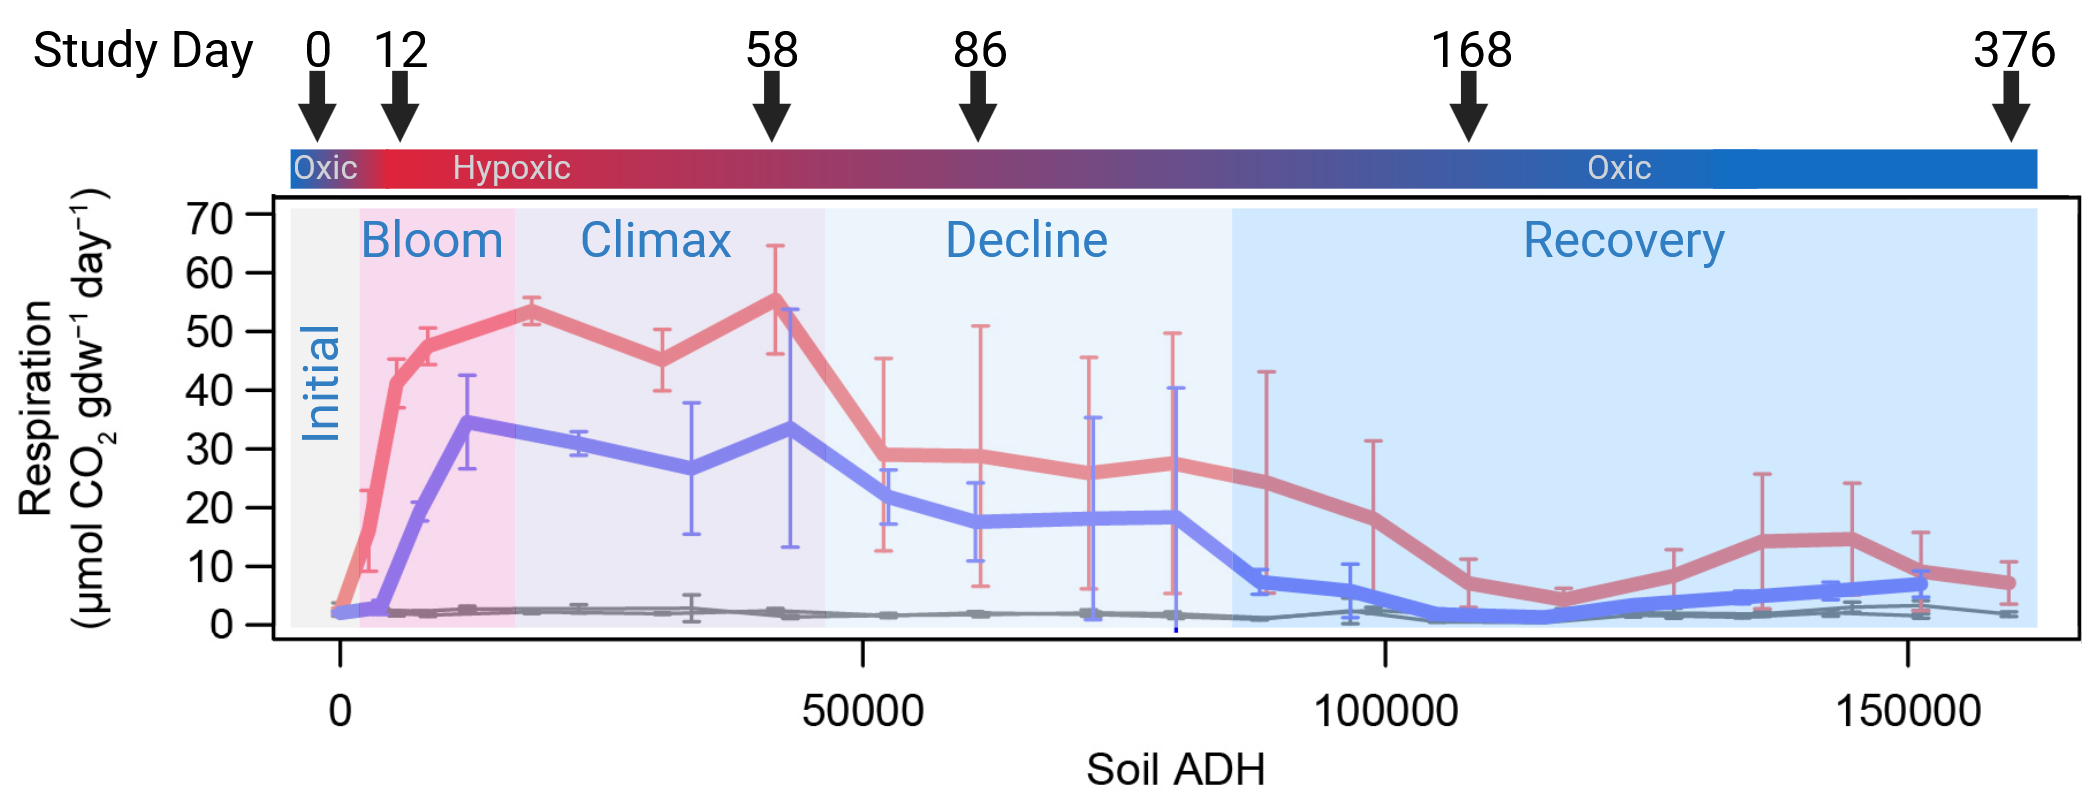
\includegraphics[width=0.95\textwidth]{../../figures/phases_MetaTsamples.png}

Figure S5. Sampling timepoints chosen for this study based key phases of
microbial activity. Lines show respiration reference data from Taylor et
al.~(2024) for both warm season (red) and cool season (blue)
decomposition trials, along with control soils (black) as a function of
soil accumulated degree hours (ADH). Oxic/hypoxic status is based on
soil oxygen data from Taylor et al.~(2024). Samples selected from the
warm season trial for the metatranscriptomic analysis in this present
study are indicated by black arrows; study day indicates days since
decomposition initiated.




\end{document}
